%=====================================================================
\chapter{Flux-surface Geometry}\label{chap.geometry}

%---------------------------------------------------------------------
\section{Introduction}\label{sec.geointro}

The goal of this chapter is to present a self-contained derivation 
and cataloguing of all geometrical quantities required for gyrokinetic 
or neoclassical simulation of plasmas with an arbitrary cross-sectional 
shape.  The method represents a refinement and generalization of 
a class of approaches which fall under the category of local 
equilibrium techniques \cite{mercier:1974}. These have a long history 
of application to ballooning mode analysis 
\cite{greene:1981,bishop:1984,miller:1998}, 
and are described in historical detail by Miller \cite{miller:1998}.  
The unified method we propose can be consistently applied 
to either a local or global equilibrium, and to flux-surfaces 
of model or general shape.  A global equilibrium, in this context, 
refers to a preexisting numerical solution of the Grad-Shafranov 
equation over the entire plasma volume, whereas a local equilibrium 
refers to Grad-Shafranov force-balance at a single surface only,
without reference to adjacent surfaces.  The latter scenario has 
proven to be a powerful tool for understanding the effect 
of plasma shape \cite{kinsey:2007,belli:2008b} on transport.

The unified approach requires that the major radius $R(\Psi_t,\theta)$ 
and elevation $Z(\Psi_t,\theta)$ along a given flux-surface 
contour are tabulated as functions of the poloidal angle $\theta$ 
(or, more generally, any parameter that labels position on the 
flux surface at constant toroidal angle).   In the local case, 
the toroidal flux, $\Psi_t$, need not be specified, and geometrical 
quantities can be evaluated up to an unknown constant (the 
so-called {\it effective field}, $\bu$), with flux-surfaces labeled 
by the {\it midplane minor radius}, $r$.  Both $\bu$ and $r$ will 
be precisely defined later.   If a global plasma equilibrium exists, 
such that the toroidal flux, $\Psi_t$, has been computed, then 
the functions $r = r(\Psi_t)$ and $\bu(r)$ can be uniquely 
determined for all $r$ (i.e., on each flux-surface).  
A special case, in which $R$ and $Z$ are approximated by up-down 
symmetric contours with finite ellipticity and triangularity (the 
so-called Miller geometry method \cite{miller:1998}), is treated 
by numerous codes worldwide \cite{dorland:2000,candy:2003,chen:2003}.
Unfortunately, the implementations of this method are not 
standardized, and documentation is typically unavailable.  
For example, in certain cases, the model shape is assumed but
Grad-Shafranov force balance is not enforced.  This gives rise
to implementation differences which significantly complicate 
code benchmarking exercises.  The challenges are further amplified 
for the consistent treatment of general (numerically-generated) 
flux-surface shape corresponding to global plasma equilibria 
\cite{xanthopoulos:2008}.  Then, not only is there an even 
greater liklihood of significant implementation difference, 
but the connections to the local limit and to the limit of 
model shape are obscured. The present work is an attempt to 
define a standard approach which unifies the treatment of 
local and global equilibria, as well as model and general
flux-surface shape.  By using a general Fourier-series 
expansion for the flux-surface shape, we show how to 
estimate the error in approximating a general closed 
contour with a model shape (often referred to as the Miller 
shape \cite{miller:1998,waltz:1999}).  We also show how to
consistently identify the local limit of a global 
equilibrium on each flux surface.  The results herein 
modify certain conventions in the local equilibrium theory 
and, further, correct a variety of sign and typographical 
errors in an earlier paper by Waltz and Miller \cite{waltz:1999}.

In Sec.~\ref{sec.coord}, we give the most general definitions
of coordinates and associated flux functions.  In Sec.~\ref{sec.local},
we use the local equilibrium method to compute all geometrical 
quantities required for gyrokinetic or neoclassical simulation 
of plasmas, given $(R,Z)$ coordinates and associated derivatives 
on a flux-surface.  We specialize these results, in 
Sec.~\ref{sec.shape}, to the specific cases of model 
(Miller) and general (Fourier series) flux-surface 
parameterizations, and provide error estimates for 
each method.  Finally, in the appendix, we give a 
large-aspect-ratio expansion of the geometry coefficients,
useful for purposes of code checking, and to make 
contact with the $s$-$\alpha$ model \cite{connor:1978}.

%---------------------------------------------------------------------
\section{Field-aligned coordinates and flux functions}
\label{sec.coord}
\subsection{Clebsch representation}

In what follows we adopt the right-handed, field-aligned 
coordinate system $(\psi,\theta,\alpha)$ together with the 
Clebsch representation \cite{kruskal:1958} for the magnetic 
field
%
\begin{equation}
\B = \nabla\alpha\times\nabla\psi
\quad\mbox{such that}\quad
\B\cdot\nabla\alpha = \B\cdot\nabla\psi = 0 
\label{eq.bc} \; .
\end{equation}

\noindent
The angle $\alpha$ is written in terms of the toroidal 
angle $\varphi$ as
%
\begin{equation}
\alpha \doteq \varphi + \nu(\psi,\theta)\; .
\label{eq.nudef}
\end{equation}

\noindent
In Eqs.~(\ref{eq.bc}) and (\ref{eq.nudef}), $\psi$ (as we will 
show) is poloidal flux divided by $2\pi$, and $\theta$ refers 
simultaneously to (a) 
an angle in the poloidal plane (at fixed $\varphi$), or 
(b) a parameterization of distance along a field line 
(at fixed $\alpha$). In these coordinates, the Jacobian is 
%
\begin{equation}
\jp \doteq \frac{1}{\nabla\psi\times\nabla\theta\cdot\nabla\alpha}
= \frac{1}{\nabla\psi\times\nabla\theta\cdot\nabla\varphi} \; . 
\label{eq.jacpsi}
\end{equation}

\noindent
Since the coordinates $(\psi,\theta,\alpha)$ and 
$(\psi,\theta,\varphi)$ form right-handed systems, 
the Jacobian $\jp$ is positive-definite.  In the latter 
coordinates, the magnetic field becomes
%
\begin{equation}
\B = \nabla\varphi\times\nabla\psi + 
\frac{\partial \nu}{\partial \theta} \nabla\theta\times\nabla\psi
\label{eq.bsalpha}
\end{equation}

\noindent 
Using the definition of the safety factor, $q(\psi)$, we 
may deduce
%
\begin{equation}
q(\psi) \doteq \frac{1}{2\pi} \int_0^{2\pi}  
\frac{\B\cdot\nabla\varphi}{\B\cdot\nabla\theta} \, d\theta 
= \frac{1}{2\pi} \int_0^{2\pi} 
   \left( -\frac{\partial \nu}{\partial \theta} \right) \, d\theta
= \frac{\nu(\psi,0)-\nu(\psi,2\pi)}{2\pi} \; .
\end{equation}

\noindent
For concreteness, we choose the following boundary conditions 
for $\nu$:
%
\begin{align}
\nu(\psi,2\pi) = &~-2\pi \, q(\psi) 
\label{eq.qdef} \; , \\
\nu(\psi,0)    = &~0 \; .
\end{align}

\noindent
By writing $\B$ in the standard form for up-down symmetric 
equilibria, 
%
\begin{equation}
\B = \nabla\varphi\times\nabla\psi + I(\psi) \nabla\varphi \; ,
\end{equation}

\noindent
we can derive the following integral for $\nu$:
%
\begin{equation}
\nu(\psi,\theta) = -I(\psi)\int_0^\theta 
\jp \left|\nabla\varphi\right|^2 d\theta\; .
\label{eq.nu}
\end{equation}

\noindent
We remark that in the case of concentric (unshifted) circular 
flux surfaces, one will obtain the approximate result 
$\nu(\psi,\theta) \sim -q(\psi)\theta$. 

\subsection{Periodicity constraints}\label{sec.period}

The periodicity requirements for physical functions are 
a potential source of confusion.  Consider a physical 
function -- for example, potential or density -- represented 
by the (real) field $z(\psi,\theta,\alpha)$.  In terms 
of the physical angle $\varphi$, we have
%
\begin{equation}
z(\psi,\theta,\alpha) = z\left(\psi,\theta,\varphi + \nu[\psi,\theta]\right) 
\end{equation}

\noindent
We impose the following topological requirements on the function $z$:

\begin{enumerate}
\item
$z$ is $2\pi/\Delta n$-periodic in $\varphi$ for fixed $\psi$ and $\theta$,
\item
$z$ is $2\pi$-periodic in $\theta$ for fixed $\psi$ and $\varphi$.
\end{enumerate}

\noindent
From this point onwards, we will refer to $\psi$ and $\chi_t$ simply 
and the poloidal and toroidal fluxes, respectively.

\subsection{Toroidal and poloidal flux}

We can start from the general forms of the toroidal and poloidal 
fluxes \cite{dhaeseleer:1991}
%
\begin{align}
\Psi_t \doteq &~\iint\limits_{S_t} \B \cdot d{\bf S} 
  = \frac{1}{2\pi} \iiint\limits_{V_t} \B \cdot \nabla\varphi \, dV \; , \\
\Psi_p \doteq &~\iint\limits_{S_p} \B \cdot d{\bf S} 
  = \frac{1}{2\pi} \iiint\limits_{V_p} \B \cdot \nabla\theta \, dV \; .
\end{align}

\noindent
Explicitly inserting the field-aligned coordinate system of the 
previous section, and differentiating these with respect to $\psi$, 
gives
%
\begin{align}
\frac{d\Psi_t}{d\psi} 
  = &~\frac{1}{2\pi} 
  \int_0^{2\pi} d\varphi \int_0^{2\pi} d\theta 
   \,\, \B\cdot\nabla\varphi \, \jp \; , \\
  = &~\frac{1}{2\pi} 
  \int_0^{2\pi} d\varphi \int_0^{2\pi} d\theta 
  \,\, \frac{\B\cdot\nabla\varphi}{\B\cdot\nabla\theta} \; , \\
  = &~2 \pi \, q(\psi) \; ,
\end{align}
\begin{align}
\frac{d\Psi_p}{d\psi} 
  = &~\frac{1}{2\pi} 
  \int_0^{2\pi} d\varphi \int_0^{2\pi} d\theta 
  \,\, \B\cdot\nabla\theta \, \jp \; , \\
  = &~\frac{1}{2\pi} 
  \int_0^{2\pi} d\varphi \int_0^{2\pi} d\theta \; , \\
  = &~2 \pi \; .
\end{align}

\noindent
Thus, $\psi$ is the poloidal flux divided by $2\pi$.  For this reason, 
it is useful to also define the toroidal flux divided by $2\pi$:
%
\begin{equation}
\chi_t \doteq \frac{1}{2\pi} \Psi_t\; .
\end{equation}

\noindent
According to these conventions, 
%
\begin{equation}
d\Psi_t = q \, d\Psi_p \quad \mbox{and} \quad
d\chi_t = q \, d\psi \; .
\end{equation}

\subsection{Flux-surface averaging and the divergence theorem}
\label{sec.fluxave}

It is also convenient to define a related 
Jacobian 
%
\begin{equation}
\jr = \frac{1}{\nabla r \times\nabla\theta\cdot\nabla\varphi} 
= \frac{\partial \psi}{\partial r} \jp \; ,
\end{equation}
%
where $r$ is the midplane minor radius.  The flux-surface average of 
a function $f$ can be expressed as
%
\begin{equation}
\fluxa(f)  \doteq \frac{1}{V^\prime} \oint \ds \,\jr \, f 
\quad\mbox{where}\quad V^\prime(r) = \oint \ds J_r \; .
\end{equation}
%
The normalizing factor $V^\prime$ is evidently the derivative 
of the flux-surface volume with respect to $r$.  The element 
of flux-surface volume can be written as $dV = dn\, dS = dr\,\ds\,\jr$
where $dS$ is the element of surface area on a flux-surface, 
and $n$ is the length along the normal vector ${\bf n}$. 
The relation between $n$ and $r$ is given by $dr = 
(\partial r/\partial n) \, dn = |\nabla r| \, dn$.
This allows one to write a form of the {\it divergence theorem}
useful for the derivation of transport equations.  Integrating 
the divergence of an arbitrary vector ${\bf A}$ over volume 
gives
%
\begin{equation}
\int dV \, \nabla \cdot {\bf A} = 
 \oint dS \, {\bf A} \cdot {\bf n} =
 \oint \frac{dS}{|\nabla r|} \, {\bf A} \cdot \nabla r =
  V^\prime(r) \, \fluxa\left( {\bf A}\cdot\nabla r \right) \; ,
\end{equation}
%
where we have used
%
\begin{equation}
\fluxa(f)  = \frac{1}{V^\prime} \oint 
 \frac{dS}{|\nabla r|} \, f  \quad\mbox{and}\quad
V^\prime(r) = \oint \frac{dS}{|\nabla r|} \; .
\end{equation}

\subsection{Additional flux functions}

%-----------------------------------------------------------
\begin{figure}
\begin{center}
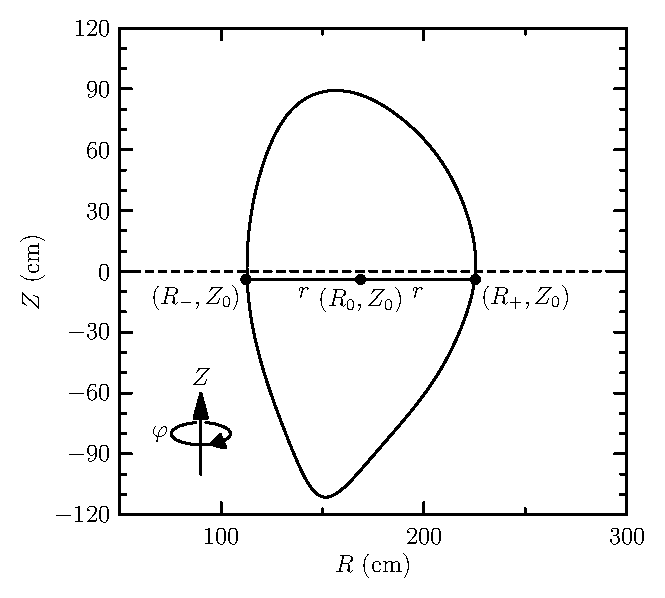
\includegraphics[scale=0.8]{figures/surf.eps}
\caption{Illustration of the centroid elevation, $Z_0$, 
the effective major radius, $R_0$, and the effective 
minor radius, $r$, for a near-separatrix flux surface 
in DIII-D.  The 
orientation of the toroidal angle, $\varphi$, is also 
indicated, such that $(R,Z,\varphi)$ is a right-handed 
system.}
\label{fig.surf}
\end{center}
\end{figure}
%-----------------------------------------------------------
%
Recall that we have assumed that the coordinates $(R,Z)$ 
of a each flux-surface are known via a one-dimensional 
parameterization (the arc length, for example).  As 
a robust measure of the flux-surface elevation, we 
use the elevation of the centroid, defined as
%
\begin{equation}
Z_0 \doteq 
 \frac{\displaystyle\oint dZ\, R Z}{\displaystyle\oint dZ\, R} \; .
\end{equation}
%
In terms of the centroid elevation, the {\it effective minor 
radius}, $r$, is defined as the half-width of the 
flux surface at the elevation, $Z_0$:
%
\begin{equation}
r \doteq \frac{R_+-R_-}{2} \; .
\label{eq.rmin}
\end{equation}
%
The quantities $R_+$ and $R_-$ are the points of intersection
of the flux surface with the line $Z=Z_0$, as illustrated in 
Fig.~\ref{fig.surf}.  We further define the {\it effective major 
radius}, $R_0 = (R_++R_-)/2$, and the {\it effective field 
strength}, $\bu$, as
%
\begin{equation}
\bu \doteq \frac{1}{r}\frac{d \chi_t}{dr} 
 = \frac{q}{r}\frac{d \psi}{dr}\; .
\end{equation}
%
The concept of an effective field was introduced by Waltz 
\cite{waltz:1999}, and represents the equivalent field that 
would be obtained if the flux surface was deformed to a 
circle with the penetrating flux held fixed.  It is 
emphasized that one must have access to a global 
equilibrium, not just the local flux-surface shape, to determine 
$\bu$.  An important feature of the unified approach is 
that the definitions of $r$ and $B_{\rm unit}$ are the 
same in both cases; that is, for both the model Grad-Shafranov 
(i.e., Miller) and general Grad-Shafranov equilibria to 
be defined shortly.

As an alternative to working with the toroidal flux directly, 
we introduce a function $\rho$, with units of length, which 
parameterizes the toroidal flux:
%
\begin{equation}
\chi_t = \frac{1}{2\pi} \int {\mathbf B} \cdot d{\mathbf S} = \frac{1}{2}
B_{\rm ref} \, \rho(r)^2 \; ,
\end{equation}
%
In the expression above, $B_{\rm ref}$ is some reference field.  
While this would normally be the vacuum toroidal field, or 
something similar, it is important to keep in mind that the 
choice is ultimately arbitrary, but by knowing $B_{\rm ref}$ 
and $\rho$, one may calculate $\chi_t$.  In terms of $\rho$, 
the area enclosed by a flux surface is approximately given 
by $A \simeq \pi\rho^2$ so long as $B_{\rm ref}$ is approximately 
equal to the on-axis toroidal field strength.  In this sense, 
$\rho$ is more intuitive, and so in certain cases more convenient, 
than $\chi_t$.

%---------------------------------------------------------------------
\section{Local Grad-Shafranov equilibria}
\label{sec.local}

The aim of this section is to compute convenient, standardized 
expressions for the common differential and integral operators 
appearing in the drift-kinetic and gyrokinetic equations.  

\subsection{Required operators}

Below we collect, in coordinate-free form, the full set of 
differential and integral operators which are to be evaluated.  
In what follows, $\wc = z_\si e B/(m_\si c)$ is the gyroradius 
of species $\si$ and $p = \sum_\si n_\si k_B T_\si$ is the total 
plasma pressure.
%
\begin{eqnarray}
\mbox{Perpendicular drift:} \nonumber\\
 \vd \cdot \nabla_\perp = 
\frac{\vp^2+\vperp^2/2}{\wc B^2} \, \B \times\nabla B \cdot \nabla_\perp
   + \frac{4\pi \vp^2}{\wc B^2} \buv \times \nabla p \cdot \nabla_\perp 
   + \frac{2\vp\omega_0}{\wc} \buv \times \mathbf{s} \cdot \nabla_\perp \; ,
\label{eq.vdotgrad}
\end{eqnarray}
\begin{equation}
\mbox{Perpendicular Laplacian:}\qquad 
\nabla_\perp^2 = \left( \nabla - \buv \buv\cdot\nabla \right)^2 \; , 
\end{equation}
\begin{equation}
\mbox{Radial gradient of eikonal:}\qquad 
  \frac{\nabla\psi}{\left|\nabla\psi\right|} 
  \cdot \nabla\alpha = \frac{\nabla\psi \cdot 
    \nabla\nu}{\left|\nabla\psi\right|} \; ,
\end{equation}
\begin{equation}
\mbox{Binormal gradient of eikonal:}\qquad 
   \buv\times\frac{\nabla\psi}{\left|\nabla\psi\right|} 
   \cdot \nabla\alpha = 
 -\frac{B}{\left|\nabla\psi\right|} \; ,
\end{equation}
\begin{equation}
\mbox{Parallel gradient:}\qquad
  \buv \cdot \nabla = \frac{1}{\jp B} \frac{\partial}{\partial\theta} \; ,
\end{equation}
\begin{equation}
\mbox{Flux-surface average:}\qquad
  \langle f \rangle = \left( \frac{dV}{d\psi} \right)^{-1}
 \oint d\theta \, d\varphi \, \jp f \; .
\label{eq.fluxave}
\end{equation}
%
The perpendicular drift operator, Eq.~(\ref{eq.vdotgrad}), is 
a sum of curvature and grad-B terms.  This particular form,
which neglects the parallel part of the drift response (see, 
for example, Eq.~(54) of Ref.~\cite{hinton:2006} or Eq.~(12) of 
Ref.~\cite{belli:2008}), is sufficient to recover all standard 
results of gyrokinetic and neoclassical theory.  In 
Eq.~(\ref{eq.fluxave}), $\langle f \rangle$ denotes the 
flux-surface average of the function $f$, and
%
\begin{equation}
\frac{dV}{d\psi} = \oint d\theta \, d\varphi \, \jp \; , 
\end{equation}
%
where $V$ is the volume enclosed by the flux surface.  In the 
drift velocity, $\s$ is the following dimensionless vector
%
\begin{equation}
\s = \frac{1}{\J B} \frac{\partial R}{\partial\theta} \ephi 
- \frac{I}{RB} \nabla R \; .
\end{equation}
%
which is discussed in more detail later.

\subsection{Metric coefficients}

Define a right-handed Cartesian coordinate system $(x,y,z)$ 
via intermediate $(R,Z,\varphi)$ coordinates as 
%
\begin{align}
x =  &~R(r,\theta) \cos(-\varphi) \; , \\
y =  &~R(r,\theta) \sin(-\varphi) \; , \\
z =  &~Z(r,\theta) \; .
\end{align}
%
In this geometry the covariant basis vectors are
%
\begin{equation}
\hat{\e}_r  \doteq \frac{\partial \rs}{\partial r}\quad, \quad\quad
\hat{\e}_\theta \doteq \frac{\partial \rs}{\partial \theta}
\quad\quad \mbox{and} \quad\quad 
\hat{\e}_\varphi \doteq \frac{\partial \rs}{\partial \varphi} \; ,
\label{eq.Bcov}
\end{equation}
%
where $\rs=(x,y,z)$.  The corresponding contravariant basis 
vectors are
%
\begin{equation}
\hat{\e}^r \doteq \nabla r \quad, \quad\quad
\hat{\e}^\theta \doteq \nabla \theta
\quad\quad \mbox{and} \quad\quad 
\hat{\e}^\varphi \doteq \nabla \varphi \; .
\label{eq.Bcont}
\end{equation}
%
With this information we can write the covariant and contravariant 
components of the metric tensor $g$ as 
$g_{ij} = \hat{\e}_i \cdot \hat{\e}_j$ and 
$g^{ij} = \hat{\e}^i \cdot \hat{\e}^j$.  It is illustrative to 
write this in matrix form as
%
\begin{equation}
g_{ij} = \left(
\begin{array}{ccc}
g_{rr} & g_{r\theta} & 0 \\
g_{r\theta} & g_{\theta\theta} & 0 \\
0      & 0      & g_{\varphi\varphi}
\end{array} \right) \; , 
\end{equation}

\noindent
where
%
\begin{align}
g_{rr} = &~\left( \frac{\partial R}{\partial r} \right)^2
+ \left( \frac{\partial Z}{\partial r} \right)^2 \; , \\
g_{r\theta} = &~\frac{\partial R}{\partial r} \frac{\partial R}{\partial\theta}
+ \frac{\partial Z}{\partial r} \frac{\partial Z}{\partial\theta} \; , \\
g_{\theta\theta} = &~\left( \frac{\partial R}{\partial\theta} \right)^2
+ \left( \frac{\partial Z}{\partial\theta} \right)^2 \; . \\
g_{\varphi\varphi} = &~R^2
\end{align}

\noindent
Since we also know that $g_{ij} \cdot g^{ij} = I$, where $I$ is the 
identity matrix, we can easily determine the contravariant counterpart 
by calculating the inverse of $g_{ij}$.  This yields
%
\begin{align}
g^{ij} = &~\frac{1}{\jr^2} \left(
\begin{array}{ccc}
g_{\theta\theta}g_{\varphi\varphi} & -g_{r\theta}g_{\varphi\varphi} & 0 \\
-g_{r\theta}g_{\varphi\varphi} & g_{rr}g_{\varphi\varphi} & 0 \\
0      & 0      & g_{rr}g_{\theta\theta}-g_{r\theta}^2
\end{array} \right) \\
\quad = &~\left(
\begin{array}{ccc}
(\nabla r)^2 & \nabla r \cdot \nabla\theta & 0 \\
 \nabla r \cdot \nabla\theta &(\nabla\theta)^2  & 0 \\
0      & 0      & (\nabla\varphi)^2
\end{array}\right) \; . 
\end{align}

\noindent
Here, the Jacobians are 
%
\begin{equation}
\jr \doteq \frac{\partial(x,y,z)}{\partial(r,\theta,\varphi)} = 
\frac{\partial \psi}{\partial r} \jp  
\quad\mbox{and}\quad
\jp \doteq \frac{\partial(x,y,z)}{\partial(\psi,\theta,\varphi)}  \; ,
\end{equation}

\noindent
where explicitly 
%
\begin{equation}
\jr = \det g_{ij} =
 R \left( 
 \frac{\partial R}{\partial r}\frac{\partial Z}{\partial\theta} - 
 \frac{\partial R}{\partial\theta}\frac{\partial Z}{\partial r}
\right) > 0 \; .
\label{eq.jac}
\end{equation}

\noindent
Metric coefficients can then be computed straightforwardly.
For example,
%
\begin{equation}
\left| \nabla r \right| = g_{\theta\theta}^{1/2}
\left[
\frac{\partial R}{\partial r}\frac{\partial Z}{\partial\theta}-
\frac{\partial R}{\partial\theta}\frac{\partial Z}{\partial r}
\right]^{-1} \; .
\end{equation}

\subsection{Mercier-Luc coordinates}

Consider a reference flux surface $\psi = \psi_s$ 
and the corresponding one-dimensional curve $\x(\arc)=(R_s,Z_s)$
defined by the intersection of that surface and 
the plane $\varphi=0$.  If we choose $\arc$ to be
the arc length along $\x$, then the tangent vector 
%
\begin{equation}
{\bf t} \doteq \frac{d\x}{d\arc} = \left( 
\frac{d R_s(\arc)}{d\arc},\frac{d Z_s(\arc)}{d\arc} 
\right)
\end{equation}
%
is a unit vector.  We can further define the unit 
tangent and unit (inward) normal vectors in terms 
of a {\it frame angle} $\ang$ \cite{guggenheimer:1977} as
%
\begin{equation}
{\bf t} \doteq \left( -\sin\ang,\cos\ang \right) \quad
\mbox{and} \quad
{\bf n} \doteq \left(-\cos\ang,-\sin\ang \right) \; .
\end{equation}
%
This definition of the frame angle is different than that 
used in Ref.~\cite{miller:1998} and \cite{waltz:1999}.
We believe the present convention is the natural choice, 
since in the circular limit we have $u=\theta$ and 
$\arc=r\theta$.  The radius of curvature, $r_c$, satisfies 
the equation
%
\begin{equation}
\frac{d{\bf t}}{d\arc} = \frac{{\bf n}}{r_c} \quad
\mbox{so that}
\quad
\frac{1}{r_c(\arc)} = \frac{d \ang}{d \arc} \; . 
\end{equation}
%
Some algebra shows that the curvature can be written as
%
\begin{equation}
r_c(\theta) = g_{\theta\theta}^{3/2} \left( 
\frac{\partial R}{\partial\theta}\frac{\partial^2 Z}{\partial\theta^2}-
\frac{\partial Z}{\partial\theta}\frac{\partial^2 R}{\partial\theta^2}
\right)^{-1} \; .
\end{equation}
%
Following Mercier and Luc \cite{mercier:1974}, we introduce 
a right-handed, orthogonal coordinate system $(\varrho,\arc,\varphi)$ 
which is defined in relation to the reference flux surface 
$\psi = \psi_s$ through
%
\begin{align}
R(r,\theta) = &~R_s(\arc) + \varrho \cos\ang \; , 
 \label{eq.rml} \\
Z(r,\theta) = &~Z_s(\arc) + \varrho \sin\ang \; . 
 \label{eq.zml}
\end{align}
%
%----------------------------------------------------------
\begin{figure}
\begin{center}
\includegraphics[scale=0.9]{figures/geom2.eps}
\caption{Mercier-Luc coordinate system.}
\label{fig.geom2}
\end{center}
\end{figure}
%----------------------------------------------------------
%
\noindent
The orientations of $\arc$ and $\ang$ are shown in 
Fig.~\ref{fig.geom2}.  The metric tensor in this 
case is diagonal, with
%
\begin{align}
g_{\varrho\varrho} = &~1 \; , \\
g_{\arc\arc} = &~\left( 1+\frac{\varrho}{r_c} \right)^2 \; , \\
g_{\varphi\varphi} = &~R^2 \; .
\end{align}
%
The Jacobian is
%
\begin{equation}
{\cal J}_\varrho = \frac{\partial(x,y,z)}{\partial(\varrho,\arc,\varphi)} 
= \frac{1}{\nabla\varrho \times \nabla\arc \cdot\nabla\varphi}
= R \left(1+\frac{\varrho}{r_c} \right) > 0 \; .
\end{equation}
%
By differentiating Eqs.~(\ref{eq.rml}) and (\ref{eq.zml}) 
with respect to $r$, and evaluating the result at $\varrho=0$,
we obtain the following identities valid {\it on the surface} 
$\psi = \psi_s$:
%
\begin{align}
\left. \frac{\partial\rho}{\partial r}\right|_{\psi=\psi_s}  
 = &~\cos\ang \, \frac{\partial R}{\partial r} 
 +\sin\ang \, \frac{\partial Z}{\partial r} \; , \\
\left. \frac{\partial\arc}{\partial r}\right|_{\psi=\psi_s} 
 = &~\cos\ang \, \frac{\partial Z}{\partial r}
 -\sin\ang \, \frac{\partial R}{\partial r} \; .
\end{align}
%
Differentiation with respect to $\theta$ yields
%
\begin{align}
\left. \frac{\partial\rho}{\partial\theta}\right|_{\psi=\psi_s}  
 = &~0 \; , \\
\left. \frac{\partial\arc}{\partial\theta}\right|_{\psi=\psi_s} 
 = &~\sqrt{ \left(\frac{\partial Z}{\partial\theta}\right)^2
+ \left(\frac{\partial R}{\partial\theta}\right)^2} = \sqrt{g_{\theta\theta}} \; .
\end{align}
%
On the surface, the Jacobian is equal to
%
\begin{equation}
\jr = \frac{R}{|\nabla r|} \frac{\partial\arc}{\partial\theta} \; .
\end{equation}


\subsection{Solution of the Grad-Shafranov equation}

The solution of Grad-Shafranov equation determines 
the poloidal flux, $\psi$, as a function of sources 
$f$ and $p$:
%
\begin{equation}
R^2 \, \nabla\cdot\left( \frac{\nabla\psi}{R^2} \right) 
= -4\pi R^2 p^\prime(\psi) - \ffp(\psi) \; .
\end{equation}
%
The lefthand side can be written as 
%
\begin{equation}
R^2 \, \nabla\cdot\left( \frac{\nabla\psi}{R^2} \right)
= \nabla^2\psi - \frac{2}{R} \, \nabla R \cdot \nabla \psi \; .
\end{equation}
%
We wish to obtain a solution valid in a neighborhood of 
$\varrho=0$ and so expand
%
\begin{equation}
\psi = \psi_s + \psi_1(\arc) \, \varrho + \psi_2(\arc) \, \varrho^2 + \cdots 
\; . \label{eq.psi}
\end{equation}
%
The required operators can then be evaluated to leading
order in $\varrho$ as
%
\begin{equation}
\nabla R = \frac{1}{h_\varrho} \frac{\partial R}{\partial\varrho}\,\hat{\e}_\varrho +
  \frac{1}{h_\arc} \frac{\partial R}{\partial\arc}\,\hat{\e}_\arc 
  \sim \hat{\e}_\varrho\,\cos\ang  - \hat{\e}_\arc\,\sin\ang 
  + \ord(\varrho) \; ,
\end{equation}
\begin{equation}
\nabla \psi = \frac{1}{h_\varrho} 
  \frac{\partial\psi}{\partial\varrho}\,\hat{\e}_\varrho +
  \frac{1}{h_\arc} \frac{\partial\psi}{\partial\arc}\,\hat{\e}_\arc 
  \sim \psi_1 \, \hat{\e}_\varrho + \ord(\varrho) \; ,
\end{equation}
\begin{align}
\nabla^2 \psi = &~\frac{1}{h_\varrho h_\arc h_\varphi} \left[ 
  \frac{\partial}{\partial\varrho}\left( \frac{h_\arc h_\varphi}{h_\varrho} 
  \frac{\partial\psi}{\partial\varrho} \right)+
  \frac{\partial}{\partial\arc}\left( \frac{h_\varrho h_\varphi}{h_\arc} 
  \frac{\partial\psi}{\partial\varrho} \right) \right] \; , \\
\qquad \sim &~\frac{\partial^2\psi}{\partial\varrho^2} 
  + \frac{\partial\psi}{\partial\varrho}\frac{1}{h_\arc h_\varphi}
\frac{\partial}{\partial\rho}\left( h_\arc h_\varphi \right) 
 + \ord(\varrho) \; ,
\end{align}
%
where $h_i \doteq \sqrt{g_{ii}}$.  Combining these results gives
%
\begin{equation}
R^2 \, \nabla\cdot\left( \frac{\nabla\psi}{R^2} \right) \sim 
\frac{\psi_1}{r_c}-\frac{\psi_1}{R_s}\cos\ang + 2\psi_2 + \ord(\varrho) \; .
\end{equation}
%
The solution for $\psi_1$ is obtained from 
%
\begin{equation}
B_p^2 = \left|\nabla\varphi\right|^2 \left|\nabla\psi\right|^2 
\sim \frac{1}{R_s^2} \left(\frac{\partial\psi}{\partial\rho}\right)^2 
+ \ord(\varrho) \; ,
\end{equation}
%
from which it is evident that 
%
\begin{equation}
\psi_1 = R_s B_{ps} \; ,
\end{equation}
%
where $B_{ps} = B_p(\psi_s)$.  The solution of the 
Grad-Shafranov equation then gives an explicit expression
for $\psi_2$:
%
\begin{equation}
\psi_2 = \frac{1}{2} \left( B_{p} \cos\ang - \frac{B_{p}R}{r_c} 
-4\pi R^2 p^\prime - \ffp \right)_{\psi = \psi_s} \; .
\end{equation}
 
\subsection{Magnetic field derivatives}

We can start with the exact expressions
%
\begin{align}
B_p^2 = &~\frac{1}{R^2} \left[ 
\left( \frac{\partial\psi}{\partial\varrho} \right)^2+
\left( \frac{1}{h_\arc} \frac{\partial\psi}{\partial \arc} 
  \right)^2 \right] \; , \\
B_t^2 = &~\left( \frac{I(\psi)}{R} \right)^2 \; .
\end{align}
%
Expanding the poloidal flux gives 
%
\begin{align}
R^2\,B_t^2 &~\sim I_s^2 + 2 \varrho \psi_1 I_s I_s^\prime 
+ \ord(\varrho^2) \; , \\
R^2\,B_p^2 &~\sim \psi_1^2 + 4 \varrho \psi_1 \psi_2 
+ \ord(\varrho^2) \; ,
\end{align}

\noindent
where $I_s = I(\psi_s)$.  Expanding $R$ and taking derivatives gives
%
\begin{align}
\frac{\partial}{\partial\varrho} B_t^2 
  &~\sim \frac{1}{R_s^2} \left( -2 \, \frac{I_s^2}{R_s}\cos\ang + 
2 I_s I_s^\prime \psi_1 \right) \; , \\
\frac{\partial}{\partial\varrho} B_p^2 
  &~\sim  \frac{1}{R_s^2} \left( -2 \, \frac{\psi_1^2}{R_s}\cos\ang + 
4 \psi_1 \psi_2 \right) \; .
\end{align}

\noindent
Adding these contributions together gives, finally:
%
\begin{equation}
\frac{\partial}{\partial\varrho} B^2 \sim 
\left( -2\,\frac{I^2}{R^3} \cos\ang - 2\,\frac{B_{p}^2}{r_c} -
8\pi R B_{p} p^\prime \right)_{\psi = \psi_s} \; .
\label{eq.brho}
\end{equation}
 
\subsection{Calculation of the eikonal function}

In order to compute radial derivatives required for 
the evaluation of the drift and Laplacian, we need to 
determine the radial dependence of $\nu$.  Using the 
expansion, Eq.~(\ref{eq.psi}), for the poloidal flux, 
together with the eikonal expansion
%
\begin{equation}
\nu = \nu_s + \nu_1(\arc) \, \varrho + \cdots \; ,
\end{equation}
%
we solve the equation 
%
\begin{equation}
\nabla\nu \times \nabla\psi = f \nabla\varphi
\label{eq.nueq} 
\end{equation}
%
order-by-order in $\varrho$.  First, an expansion of 
the gradients yields
%
\begin{align}
\nabla\psi &~\sim \left( \psi_1+2\varrho \psi_2 \right) \nabla\varrho 
+ \varrho \frac{\partial\psi_1}{\partial\arc} \nabla\arc +\ord(\varrho^2) \; , \\
\nabla\nu &~\sim \nu_1 \nabla\varrho + \left(
\frac{\partial \nu_s}{\partial\arc}+\varrho\frac{\partial \nu_1}{\partial\arc}
\right) \nabla\arc +\ord(\varrho^2) \; .
\end{align}

\noindent
Replacing these formulae into Eq.~(\ref{eq.nueq}) and dotting with 
$\nabla\varphi$ yields
%
\begin{equation}
-\frac{\partial\nu_s}{\partial\arc} \psi_1 + \varrho
\left( \nu_1 \frac{\partial\psi_1}{\partial\arc}-
       \frac{\partial\nu_1}{\partial\arc} \psi_1 
       - 2\frac{\partial\nu_s}{\partial\arc} \psi_2 \right) \sim
\frac{I_s+\varrho I_s^\prime \psi_1}{R_s+\varrho\cos\ang}
\left( 1+\frac{\varrho}{r_c}\right) \; .
\end{equation}
\noindent
At each order in $\varrho$, we have
%
\begin{align}
\ord(1):\quad &~ -\frac{\partial\nu_s}{\partial\arc}\psi_1 
 = \frac{I_s}{R_s} \; , \\
\ord(\varrho):\quad &~ -\psi_1 \frac{\partial}{\partial\arc} \left(
\frac{\nu_1}{\psi_1} \right) 
 = 2 \, \frac{\partial \nu_s}{\partial\arc} \frac{\psi_2}{\psi_1}
  + \frac{I_s^\prime}{R_s} + \frac{I_s}{R_s r_c \psi_1} 
 - \frac{I_s\cos\ang}{R_s^2 \psi_1} \; .
\end{align}

\noindent
Thus, the solution for $\nu_s$ is
%
\begin{equation}
\nu_s(\arc) = -\int_0^\arc \darcp \, I_s \; .
\end{equation}

\noindent
Some additional algebra shows that
%
\begin{equation}
\nu_1(\arc) = R_s(\arc) B_{ps}(\arc) \left[
D_0(\arc) + D_1(\arc) \, \ffp + D_2(\arc) \, p^\prime 
\right] \; ,
\end{equation}

\noindent
where the $D_i$ integrals are:
%
\begin{align}
D_0 = &~ -\int_0^\arc \darcp \left( 
\frac{2}{r_c R_s B_{ps}} - \frac{2\cos\ang}{R_s^2 B_{ps}} \right) I_s \\
D_1 = &~ -\int_0^\arc \darcp \left( 
\frac{B^2}{B_{ps}^2} \right) \frac{1}{I_s} \; , \\
D_2 = &~ -\int_0^\arc \darcp \left( 
\frac{4\pi}{B_{ps}^2} \right) I_s \; .
\end{align}

\noindent
We want to eliminate $\ffp$ in favour of $q^\prime$.  Writing 
$\arc(2\pi) \doteq L$, and expanding Eq.~(\ref{eq.qdef}), we 
find 
%
\begin{equation}
-2\pi (q_s + q_s^\prime \varrho \psi_1) \sim 
\nu_s(L) + \varrho \nu_1(L) + \ord(\varrho^2) \; .
\end{equation}

\noindent
Therefore, we have the connection
%
\begin{equation}
-2\pi \, q_s^\prime = D_0(L) + D_1(L) \, \ffp + D_2(L) \, p^\prime \; .
\end{equation}

\subsection{Gyrokinetic drift velocity in Mercier-Luc coordinates}

In this case, we work out the dominant part of the drift 
operator acting on a function $f(\psi,\theta,\alpha)$.
This limit is appropriate for standard gyrokinetics.
We proceed by simplifying Eq.~(\ref{eq.vdotgrad}) in the 
Miller equilibrium case by beginning from the Mercier-Luc 
representation.  On the surface $\psi = \psi_s$ we have
%
\begin{equation}
\B_s = B_{ps} \nabla\arc + I_s \nabla \varphi \; . 
\label{eq.bsurf}
\end{equation}

\noindent
Note that Eq.~(\ref{eq.bsurf}) cannot be used to obtain 
$\partial B/\partial\psi$ because the limit $\varrho \rightarrow 0$ 
has already been taken.  To evaluate $\nabla B$, we must write
%
\begin{equation}
\nabla B = \frac{\partial B}{\partial\varrho} \nabla\varrho +
\frac{\partial B}{\partial\arc} \nabla\arc \; ,
\end{equation}
%
and then make use of Eq.~(\ref{eq.brho}).  Taking the cross product 
of the above two quantities gives
%
\begin{equation}
\B_s \times \nabla B = 
-B_{ps} \frac{\partial B}{\partial\varrho} 
 \nabla\varrho\times\nabla\arc
+I_s \frac{\partial B}{\partial\varrho} 
 \nabla\varphi\times\nabla\varrho
+I_s \frac{\partial B}{\partial\arc} 
 \nabla\varphi\times\nabla\arc \; .
\label{eq.mldrift}
\end{equation}

\noindent
Then, the perpendicular gradient operator, accurate to $\ord(\varrho)$, 
can be written as 
%
\begin{equation}
\nabla_\perp \sim \nabla\varrho \, \frac{\partial}{\partial\varrho}+
\left( \nabla\varphi + \frac{\partial \nu_s}{\partial\arc} \, \nabla\arc 
         + \nu_1 \nabla\varrho + \ord(\varrho) \right) 
\frac{\partial}{\partial\alpha} \; .
\label{eq.nabla}
\end{equation}

\noindent
The final result, valid on the surface $\psi = \psi_s$, is 
%
\begin{equation}
\B \times \nabla B \cdot \nabla = 
-I_s B_{ps} \, \frac{\partial B}{\partial\arc} 
\frac{\partial}{\partial\psi} + \left( 
-\frac{B^2}{R_s B_{ps}}\frac{\partial B}{\partial\varrho}
-\frac{I_s \nu_1}{R_s}\frac{\partial B}{\partial\arc} \right) 
\frac{\partial}{\partial\alpha} \; .
\end{equation}

\subsection{Perpendicular Laplacian in Mercier-Luc coordinates}

To evaluate the perpendicular Laplacian, we square Eq.~(\ref{eq.nabla}) 
and simplify, where it is sufficiently accurate to ignore variation of 
coefficients
%
\begin{equation}
\nabla_\perp^2 \sim \frac{\partial^2}{\partial \varrho^2}
+ 2 \nu_1  \frac{\partial}{\partial \varrho} \frac{\partial}{\partial \alpha}
+ \left[ \frac{1}{R^2} + \nu_1^2 + \left( \frac{\partial \nu_0}{\partial\arc} 
\right)^2 \right] \frac{\partial^2}{\partial \alpha^2} \; .
\end{equation}

\subsection{Coriolis drift terms}

Some algebra show that 
%
\begin{equation}
\buv \times \mathbf{s} \cdot \nabla_\perp = 
-\sin\ang\frac{\partial}{\partial\rho}
+ \left(\frac{I}{R^2B_p} \cos\ang - \nu_1 \sin\ang \right)
\frac{\partial}{\partial\alpha} \; ,
\end{equation}
%
where we have used the relation
%
\begin{equation}
\sin\ang = - \frac{\partial R}{\partial\theta} \left( 
\frac{\partial\ell}{\partial\theta} \right)^{-1} \; .
\end{equation}

\subsection{Detailed catalogue of shape functions}\label{sec.catalog}

For convenience, we give a complete summary of the 
equations needed to compute all the relevant shape functions.
In the expressions below, $R$ and $Z$ are taken to be 
functions of $r$ and $\theta$, and the subscript $s$ can be 
safely omitted. 
%
\begin{equation}
\frac{\partial\arc}{\partial\theta} = \sqrt{\left( 
  \frac{\partial R}{\partial\theta} \right)^2
+ \left( \frac{\partial Z}{\partial\theta} \right)^2} \; ,
\end{equation}
%
\begin{equation}
\jr = R \left( 
 \frac{\partial R}{\partial r}\frac{\partial Z}{\partial\theta} - 
 \frac{\partial R}{\partial\theta}\frac{\partial Z}{\partial r}
\right)\; ,
\end{equation}
%
\begin{equation}
\left| \nabla r \right| = \frac{R}{\jr}
  \frac{\partial\arc}{\partial\theta} \; ,
\end{equation}
%
\begin{equation}
r_c(\theta) = \left(\frac{\partial\arc}{\partial\theta}\right)^3 \left( 
\frac{\partial R}{\partial\theta}\frac{\partial^2 Z}{\partial\theta^2}-
\frac{\partial Z}{\partial\theta}\frac{\partial^2 R}{\partial\theta^2}
\right)^{-1} \; ,
\end{equation}
%
\begin{equation}
\frac{I(r)}{\bu} = 2\pi \, r \left( \int_0^L \darce \right)^{-1} \; , 
\label{eq.fobu}
\end{equation}
%
\begin{equation}
\frac{B_t(r,\theta)}{\bu(r)} = \frac{I}{R\bu}\; ,
\end{equation}
%
\begin{equation}
\frac{B_p(r,\theta)}{\bu(r)} = \frac{r}{R}\frac{|\nabla r|}{q} \; ,
\end{equation}
%
\begin{equation}
\frac{B(r,\theta)}{\bu(r)} = \mathrm{sgn}(\bu) \, \sqrt{
 \left(\frac{B_p}{\bu}\right)^2+\left(\frac{B_t}{\bu}\right)^2} \; ,
\end{equation}
%
\begin{equation}
\msin(r,\theta) \doteq \frac{B_t}{B} 
\left(\frac{R_0}{B}\frac{\partial B}{\partial\arc}\right) \; ,
\end{equation}
%
\begin{equation}
\mcos(r,\theta) \doteq -\frac{R_0}{B}\frac{\partial B}{\partial\varrho} 
= \mcosa + \mcosb \; , 
\end{equation} 
%
\begin{equation}
\mcosa(r,\theta) = \frac{B_t^2}{B^2}\frac{R_0}{R} \cos u +
\frac{B_p^2}{B^2}\frac{R_0}{r_c} \; ,
\end{equation}
%
\begin{equation}
\mcosb(r,\theta) = -\frac{1}{2}\frac{\bu^2}{B^2} R_0 
 \, |\nabla r| \, \beta^* \; ,
\end{equation}
%
\begin{equation}
\usin(r,\theta) = \sin\ang \; ,
\end{equation}
%
\begin{equation}
\ucos(r,\theta) = \frac{B_t}{B} \cos\ang \; ,
\end{equation}
%
\begin{equation}
E_1(r,\theta) = 2 \int_0^{\arc(\theta)} \darce \frac{B_t}{B_p} 
\left( \frac{r}{r_c} - \frac{r}{R} \cos u \right)
\end{equation}
%
\begin{equation}
E_2(r,\theta) = \int_0^{\arc(\theta)} \darce \left( 
\frac{B^2}{B_p^2} \right) \; ,
\end{equation}
%
\begin{equation}
E_3(r,\theta) = \frac{1}{2} \int_0^{\arc(\theta)} 
 \frac{d\arc^\prime}{R} \frac{B_t}{B_p} \left( 
 \frac{\bu^2}{B_p^2} \right) \; ,
\end{equation}
%
\begin{equation}
f^*(r) = \frac{1}{E_2(r,2\pi)} \left[ 2\pi \frac{q s}{r} - 
\frac{1}{r} E_1(r,2\pi) + \beta^*E_3(r,2\pi) \right] 
\end{equation}
%
\begin{equation}
\mk(r,\theta) \doteq -\left( \frac{R B_p}{B} \right) \nu_1 
= \frac{R B_p}{B} |\nabla r| 
\left( \frac{1}{r} E_1 + f^* E_2 - \beta^* E_3 \right) 
\end{equation}
%
\begin{equation}
\mq(r,\theta) \doteq \frac{1}{q} \left(\frac{rB}{R B_p}\right) \; ,
\end{equation}
%
\begin{equation}
\mt(r,\theta) \doteq \frac{\jp B}{q R_0} 
 = \frac{B}{\bu}\frac{R}{R_0} \frac{1}{r|\nabla r|} 
   \frac{\partial\arc}{\partial\theta} \; . 
\end{equation}

\subsection{Required operators in terms of shape functions}
\label{sec.shapefun}

\begin{eqnarray}
\mbox{Perpendicular drift:} & \nonumber \\
\vd \cdot \nabla_\perp = 
-i k_\theta \,\mq \left( \frac{\vp^2+\mu B}{\wc R_0} \right) \, \,
\left[ \mcosa + \mcosb + \mk \, \msin \right] & \nonumber \\ 
\qquad +i k_\theta \,\mq \left( \frac{\vp^2}{\wc R_0} \right) \, \,  
 \mcosb 
-\left( \frac{\vp^2+\mu B}{\wc R_0} \right) \, |\nabla r| \,
\msin \, \frac{\partial}{\partial r} \; , & \nonumber \\
\qquad -i k_\theta \,\mq \left( \frac{2\vp \omega_0 R_0}{\wc R_0} \right) \, \,  
 \left[ \ucos + \mk \, \usin \right]
-\left( \frac{2\vp\omega_0 R_0}{\wc R_0} \right) \, |\nabla r| \,
\usin \, \frac{\partial}{\partial r} \; , \label{eq.mdrift} &
\end{eqnarray}
\begin{eqnarray}
\mbox{Perpendicular Laplacian:} & \nonumber \\
\nabla_\perp^2 = \left| \nabla r \right|^2 \frac{\partial^2}{\partial r^2} 
+ 2 i \mk k_\theta \mq \left| \nabla r \right| \frac{\partial}{\partial r} 
- k_\theta^2 \mq^2 \left( 1+\mk^2 \right) \; , &
\end{eqnarray}
\begin{equation}
\mbox{Radial gradient of eikonal:}\qquad
n \, \frac{\nabla\psi}{\left|\nabla\psi\right|} \cdot \nabla\alpha = 
-k_\theta \, \mq \mk \; , 
\end{equation}
\begin{equation}
\mbox{Binormal gradient of eikonal:}\qquad
n \, \buv\times\frac{\nabla\psi}{\left|\nabla\psi\right|} \cdot 
 \nabla\alpha =
- k_\theta \, \mq \; ,
\end{equation}
\begin{equation}
\mbox{Parallel gradient:}\qquad
\buv \cdot \nabla = \frac{1}{G_\theta}\frac{1}{q R_0} 
 \frac{\partial}{\partial\theta} \; ,
\end{equation}
\begin{equation}
\mbox{Flux-surface average:}\qquad
\langle f \rangle = 
 \frac{\displaystyle \int_0^{2\pi} d\theta \, \frac{\mt}{B} \, f(\theta)}{%
       \displaystyle \int_0^{2\pi} d\theta \, \frac{\mt}{B}} \; .
\end{equation}
%
Above, we have introduced the binormal wavenumber, 
$k_\theta = i (q/r) \partial/\partial\alpha$.  

\subsection{Pressure-gradient effects in the drift velocity}

In cases where compressional magnetic perturbations are neglected, 
one may also wish to ignore finite-pressure effects in the drift 
velocity \cite{waltz:1999}.  This is done by setting $\mcosb = 0$ 
in Eq.~(\ref{eq.mdrift}). 

\clearpage

\section{Specification of the plasma shape}
\label{sec.shape}

It is assumed throughout that we have access to a global
equilibrium for which the poloidal and toroidal fluxes 
are known over the entire range of $r$.  Then, we consider 
two general ways in which to specify the plasma shape
via a closed contour in the $(R,Z)$ plane:  
(1) a model parameterization, and 
(2) a general Fourier expansion.

In addition to the plasma shape, we also need to know 
the plasma pressure gradient, which we will define 
via the effective inverse beta-gradient scale length:
%
\begin{equation}
\beta^*(r) \doteq -\frac{8\pi}{\bu^2} \frac{\partial p}{\partial r} > 0 \; .
\end{equation}
%
The safety factor $q=d\psi/d\chi_t$ and the magnetic shear 
$s=(r/q) dq/dr$ can be obtained directly via numerical differentiation.

\subsection{Model flux-surface shape}

A popular model for the flux-surface shape in $(R,Z)$
coordinates was introduced by Miller \cite{miller:1998}.  We 
generalize that model to include the effects of elevation 
and squareness.  In particular, finite elevation is required 
very close to $r=0$, where the flux surface may lie entirely 
above the midplane at $Z=0$.  Specifically, let
%
\begin{align}
R(r,\theta) = &~R_0(r) 
 + r \cos(\theta + \arcsin\delta \sin\theta) \; , \\
Z(r,\theta) = &~Z_0(r) 
 + \kappa(r) r \sin(\theta + \zeta \sin 2\theta) \; ,
\end{align}
%
where $\kappa$ is the elongation, $\delta$ is the triangularity, 
$\zeta$ is the squareness and $Z_0$ is the elevation \cite{turnbull:1999}.
In order to evaluate the required quantities 
$\partial R/\partial r$ and $\partial Z/\partial r$, we 
also need to know the radial derivatives of $R_0$, $Z_0$, 
$\delta$, $\kappa$ and $\zeta$.  To this end, we define 
the associated shape functions 
%
\begin{equation}
s_\kappa \doteq \frac{r}{\kappa} \frac{\partial\kappa}{\partial r} \; , \quad
s_\delta \doteq r \, \frac{\partial\delta}{\partial r} \; , \quad
s_\zeta \doteq r \, \frac{\partial\zeta}{\partial r} \; .
\end{equation} 
% 
Note that this definition of $s_\delta$ differs slightly from 
Refs.~\cite{miller:1998} and \cite{waltz:1999}.
Thus, to compute the shape functions for the flux-surface at 
$r$ according to this model, we require the 10 parameters
%
\begin{equation}
\left\{R_0,\frac{dR_0}{dr},Z_0,\frac{dZ_0}{dr},
\kappa,s_\kappa,\delta,s_\delta,\zeta,s_\zeta\right\} \; .
\end{equation}

\subsection{General flux-surface shape}

In this case the flux-surface shape is an expansion of the form
%
\begin{align}
R(r,\theta) = &~\frac{1}{2} \, a^R_0(r) + \sum_{n=1}^N 
 \left[ a^R_n(r) \cos(n\theta) + b^R_n(r) \sin(n\theta) \right] \; , \\
Z(r,\theta) = &~\frac{1}{2} \, a^Z_0(r) + \sum_{n=1}^N 
 \left[ a^Z_n(r) \cos(n\theta) + b^Z_n(r) \sin(n\theta) \right] \; .
\end{align}
%
Here, $N$ is an integer which evidently controls the 
accuracy of the expansion, and is in principle arbitrary.
If $(R,Z)$ are known as functions of arc length, then one
can simply set $\theta = 2\pi \arc/L$.
To compute the shape functions for the flux-surface at $r$, 
we require the $8(N+1)$ parameters
%
\begin{equation}
\left\{a^R_n,b^R_n,a^Z_n,b^Z_n,
\frac{da^R_n}{dr},\frac{db^R_n}{dr},
\frac{da^Z_n}{dr},\frac{db^Z_n}{dr}\right\} \; .
\end{equation}

\subsection{A measure of the error}

It is beyond the scope of the present paper to give 
a detailed assessement of the error in neoclassical or 
turbulent transport calculations caused by errors in 
the flux-surface shape.  Nevertheless, we can define 
the error in the flux-surface approximation of the 
discrete data $\{ R_i,Z_i \}_{i=1}^{n_d}$ as
%
\begin{equation}
\varepsilon \doteq \frac{1}{n_d \, r} \sum_{i=1}^{n_d} 
\min_\theta \sqrt{\left[ R(\theta)-R_i \right]^2 
+\left[ Z(\theta)-Z_i \right]^2} \; .
\label{eq.metric}
\end{equation}
%
Figure \ref{fig.error} shows the flux-surface fitting 
error for DIII-D discharge 132010.  
This discharge is part of a series of experiments
designed to accurately measure profiles across
the entire confined plasma, including the edge
barrier region.  Discharge 132010 is
a standard DIII-D H-mode plasma, with typical values
of the magnetic field ($B_t=2.1T$), current ($I_p=1.2MA$),
elongation ($\kappa = 1.8$) and triangularity ($\delta = 0.3$).
The width of the edge barrier ($\sim3\%$ in $r/a$), height of the
edge barrier ($\sim11 kPa$), and global pressure ($\beta_N \sim 2$)
are all fairly typical of DIII-D H-Modes.
The Grad-Shafranov 
equillbrium was computed by EFIT using a $129 \times 129$ 
mesh, and then mapped to very-high-resolution $(R,Z)$-contours 
(400 flux surfaces, each with 512 points equally-spaced 
in arc length along the surface) using the ELITE code.  
The Miller-type model equilibrium is seen to be significantly 
less accurate, according to the metric defined in Eq.~\ref{eq.metric},
at all radii than even the $N=4$ Fourier expansion (red curve).  
The $N=8$ (solid black curve) and $N=12$ (green curve) results 
are also shown.  In the region $r/a < 0.4$, 
the accuracy of the Fourier expansion probably exceeds the 
accuracy of the original equilibrium solution, and is 
therefore limited by it.  This result shows that $N>12$
is probably a good default choice for $N$.  A further
comparison of actual flux surface shapes at $r/a=0.99$
(i.e., very close to the separatrix) is shown in 
Fig.~\ref{fig.surf23}.
%
\begin{figure}
\begin{center}
\includegraphics[scale=0.8]{figures/error.eps}
\caption{Error, $\varepsilon$, in the flux-surface 
fits for DIII-D discharge 132010.  The Miller-type 
model equilibrium is seen to be significantly less 
accurate at all radii than even the $N=4$ Fourier 
expansion (red curve).  The 
$N=8$ (solid black curve) and $N=12$ (green curve) 
results are also 
shown.  In the region $r/a < 0.4$, the accuracy of
the Fourier expansion probably exceeds the accuracy 
of the original equilibrium solution, and is therefore 
limited by it.}
\label{fig.error}
\end{center}
\end{figure}
%
\begin{figure}
\begin{center}
\includegraphics[scale=0.8]{figures/surf2.eps}
\hskip 0.1in
\includegraphics[scale=0.8]{figures/surf3.eps}
\caption{Comparison of exact flux-surface (dashed curve) to 
parameterized (left) and general Fourier expansion (right)
at $r/a=0.99$.}
\label{fig.surf23}
\end{center}
\end{figure}

For core plasma parameters, our limited experience is 
that the difference, with respect to linear growth rates, 
between general and model flux-surfaces is insignificant 
in moderately-shaped DIII-D plasmas (roughly $5\%$ at 
$r/a = 0.9$, and less than that deeper in the core).  
However, this relies on the accuracy of the fitting procedure 
used to obtain the model parameters $\kappa$, $\delta$, etc.  
If the model flux-surface shape is poorly calculated, the 
absolute error can be significant.

\clearpage
\section*{Appendix A:  Large-aspect-ratio expansion}

Consider a shifted-circle (Shafranov) flux-surface shape:
%
\begin{align}
R(r,\theta) = &~R_0+\Delta(r)+r \cos\theta \; , \\
Z(r,\theta) = &~r \sin\theta \; . 
\end{align}

\noindent
Let $\Delta(r) = a r^2/(2 R_0)$ be the Shafranov shift, with $a$ 
an ${\cal O}(1)$ constant, so that $\partial \Delta/\partial r 
= a\,(r/R_0)$.  It is instructive to calculate the shape 
functions as Taylor series in the small parameter $r/R_0$.  
To first order in $r/R_0$, we find
%
\begin{equation}
|\nabla r | \sim 1-a\,\frac{r}{R_0} \cos\theta \; ,
\end{equation}
%
\begin{equation}
\frac{B_t(r,\theta)}{\bu(r)} \sim 1-\frac{r}{R_0} \cos\theta \; ,
\end{equation}
%
\begin{equation}
\frac{B_p(r,\theta)}{\bu(r)} \sim \frac{r}{q R_0} 
  \left[ 1- (a+1)\frac{r}{R_0}\cos\theta \right] \; ,
\end{equation}
%
\begin{equation}
\frac{B(r,\theta)}{\bu(r)} \sim 1-\frac{r}{R_0}\cos\theta \; ,
\end{equation}
%
\begin{equation}
\msin(r,\theta) \sim \sin\theta 
  \left[ 1 - \frac{r}{R_0} \cos\theta \right] \; ,
\end{equation}
%
\begin{equation}
\mcosa(r,\theta) \sim \cos\theta - \frac{r}{R_0} \left( 
  \cos^2\theta-\frac{1}{q^2} \right) \; ,
\end{equation}
%
\begin{equation}
\mk(r,\theta) \sim s \theta - q^2 R_0 \beta^* \sin\theta + \
  \Theta_1 \frac{r}{R_0} \; ,
\end{equation}
%
\begin{equation}
\mq(r,\theta) \sim 1+ (a-1) \frac{r}{R_0} \cos\theta \; , 
\end{equation}
%
\begin{equation}
\mt(r,\theta) \sim 1+ a\,\frac{r}{R_0} \cos\theta \; .
\end{equation}
%
Here, $\Theta_1$ is the function
%
\begin{equation}
\Theta_1 = (1-2 a)s \theta \sin\theta + \sin\theta \left[
(3a-1)s-2(1+a)+\frac{1}{2}(a-3) q^2 R_0 \beta^* \cos\theta\right] \; .
\end{equation}
%
Since the formulae do not represent an exact Grad-Shafranov 
equilibrium, but rather an equilibrium accurate only first order 
in $r/R_0$, they should not be used for simulation purposes.
However, they can be used to provide a convenient asymptotic 
check of the numerical routines used to compute the shape 
functions in the general case.   

Finally, for completeness, we can make contact with the popular 
$s$-$\alpha$ equilibrium model \cite{connor:1978}.  First, recall 
that 
%
\begin{equation}
\alpha_{\rm MHD} \doteq q^2 R_0 \beta^* = - q^2 R_0 \frac{8 \pi}{\bu^2} 
\frac{dp}{dr} \; .
\end{equation} 
%
To recover the usual $s$-$\alpha$ formulae, we must take the limit 
$r/R_0 \rightarrow 0$ in all the expressions above, except for $B$, 
which is taken to be $B/\bu = R_0/R$.  
Evidently, the result is not a Grad-Shafranov equilibrium
(not even to first order in $r/R_0$).  In practice, simulation 
results obtained using a model circular equilibrium (sometimes 
called a ``Miller circle'') can differ significantly from the 
corresponding $s$-$\alpha$ result.  For example, Kinsey 
\cite{kinsey:2007} has shown that the nonlinear electron energy 
flux increases by more than a factor of 1.5 when using a Miller 
circle instead of $s$-$\alpha$ geometry. 

\clearpage
\section*{Appendix B: Translation to GS2 Geometry Variables}

The normalizing magnetic field in GS2, $B_{T0}$, is defined as
%
\begin{equation}
I(\psi) = R B_t \doteq R_{\rm GEO} B_{T0} \; ,
\end{equation}
%
where $R_{\rm GEO}$ is a reference radius (input).  For simplicity, let's assume that 
$R_{\rm GEO} = R_0$ (this appears to be a typical choice), in which case we can then relate 
$B_{T0}$ to $\bu$ according to
%
\begin{equation}
\frac{\bu}{B_{T0}} = R_0 \left( \frac{I}{\bu} \right)^{-1} \; ,
\end{equation}
%
where $I/\bu$ is given by Eq.~(\ref{eq.fobu}).  Explicitly, we can write this as
%
\begin{align}
\frac{\bu}{B_{T0}} = &~\frac{R_0}{2\pi r} \int_0^{2\pi} \frac{d\theta}{R} 
\left( 
 \frac{\partial R}{\partial r}\frac{\partial Z}{\partial\theta} - 
 \frac{\partial R}{\partial\theta}\frac{\partial Z}{\partial r}
\right) \; , \label{eq.bex} \\
\simeq &~ \kappa\left( 1+\frac{s_\kappa}{2}-\frac{1}{2}\frac{dR_0}{dr} \frac{r}{R_0} \right) \; .
\label{eq.bap}
\end{align}
%
Whereas Eq.~(\ref{eq.bex}) is exact, Eq.~(\ref{eq.bap}) is approximate and is given 
here only as an intuitive aid.  In practice the required integral is computed to high 
accuracy by GYRO and the result available in the normalized GEO interface variable 
{\tt GEO\_f}.  Specifically,
%
\begin{equation}
\frac{\bu}{B_{T0}} = \frac{R_0}{a} \frac{1}{\tt GEO\_f} \; .
\end{equation}
